\renewcommand\evenpagerightmark{{\scshape\small Filière Work for Centrale}}
\chapter[Partie filière]%
{Partie filière}
\label{Partie filière}

\section{Partie filière}

\section{Besoins industriels d'Air Liquide}

Air Liquide utilise la combustion pour produire des gaz industriels comme l'hydrogène ou le monoxyde de carbone. Ces gaz sont les matières premières indispensables à bon nombres d'industries chimiques, notamment la pétrochimie. L'activité première d'Air Liquide étant de vendre des contrats de l'oxygène qu'elle produit, l'activité combustion d'Air Liquide ne se fait pas à l'air mais avec de l'oxygène (on a retiré l'azote de l'air) : c'est le principe d'oxycombustion. Cette technologie permet également d'atteindre des températures plus élevées qu'à l'air, d'améliorer le rendement du combustible, ainsi que de limiter significativement les émissions polluantes.
    
Les fours produisant ce mélange monoxyde de carbone/hydrogène sont appelés fours AutoThermal Reforming (ATR). Ils ont été dimensionnés par la société Lurgi, rachetée par Air Liquide en 2007. Aujourd'hui, les règles de dimensionnement des fours ATR sont mal maîtrisées. L'ingénierie n'est pas encore prédictive et la conception manque d'outils pour dimensionner les brûleurs. Air Liquide veut donc davantage maîtriser les process dans le but de :
\begin{itemize}
\item Augmenter la production en sortie de gaz
\item Maîtriser davantage les rejets
\item Diminuer le coût de dimensionnement des fours (CAPEX) ou augmenter l'efficacité de la conversion du fuel en gaz de synthèse (OPEX)
\item Obtenir des gaz de meilleurs qualités
\end{itemize}

Dans ce but, un pilote a été construit en 2004 à Freiberg. De nombreux tests ont été conduits sur ce brûleur et ces données sont le point de départ du stage.


A travers mon stage stage, Air Liquide désire :
\begin{itemize}
\item Obtenir des règles de dimensionnement pour les brûleur ATR : lois d'échelles par des nombres adimensionnés adaptés, justifier les choix technologiques de Lurgi
\item Comprendre le comportement des flammes et les mécanismes responsables
\item Donner de la visibilité à la recherche numérique, qui manque aujourd'hui cruellement de données expérimentales pour justifier les modèles
\end{itemize}



\subsection{L'ATR au sein de la R\&D aux loges}

 Peu de travaux ont été conduits sur les fours ATR, et la majorité concerne l'équipe de mathématiques appliquées. Les volumes de fours ATR vendus dans le monde sont aujourd'hui faibles mais sont toujours des investissements conséquents. Air Liquide s'intéresse de nouveaux aux ATR depuis le rachat de Lurgi mais l'appropriation et la remise en questions de la conception des ATR nécessite du temps.

\section{Déroulé et plans du stage}


En terme de gestion de projet, mon stage s'insère dans un programme de recherche plus général : la chaire Oxytec a été créée entre Air Liquide et le laboratoire EM2C de Centrale pour investiguer le comportement des flammes d'Air Liquide, qui sont très atypiques (haute pression, combustion de l'oxygène, éventuelles dilutions...). La chaire a financé six thèses dont l'objectif final est de fournir des outils numériques et un banc d'essai de haute précision permettant de reproduire et observer les flammes industrielles (ce qui requiert des moyens très conséquents et n'a jamais pu être réalisé auparavant). Au sein de ce programme, mon stage amorce la réflexion sur les véritables brûleurs utilisés dans les procédés Air Liquide. Il est en très forte relation avec la dernière thèse que le projet Oxytec a prévue, thèse pour laquelle je suis aujourd'hui le candidat d'Air Liquide et du EM2C.

Il est nécessaire de comprendre pourquoi l'étude des flammes n'est pas encore maîtrisée aujourd'hui :
\begin{itemize}
\item D'un point de vue numérique, résoudre les équations d'une flamme requiert des moyens de calculs inaccessibles même aux plus grands super-calculateurs mondiaux.
\item D'un point de vue expérimental, étudier une flamme de taille industrielle (pression et puissance très élevées : 40 bar, 5MW) est à la fois prohibitif dans le prix et inaccessible expérimentalement puisque il est impossible de placer des capteurs dans des flammes industrielles
\end{itemize}

La stratégie est donc de recourir aux lois d'échelles : par un dimensionnement judicieux, on veut montrer qu'on peut se rapporter à des flammes de laboratoires (néanmoins très importantes), mais qu'on peut analyser. C'est le premier objectif de mon stage : retrouver la flamme du pilote industriel de Freiberg par l'analyse des phénomènes.

Si cet objectif est rempli, alors on aura la légitimité pour étudier l'influence de paramètres qui n'ont vraisemblablement pas été étudiés lors de la conception des brûleurs.Par exemple, en changeant simplement certains débits judicieusement ou le design du brûleur, on espère pouvoir piloter les caractéristiques de la flamme.

\subsection{Ce qui a été réalisé}

J'ai été confronté dès le début à toutes les contraintes d'ordre industriel sur lesquels j'avais assez peu d'emprise : les délais pour lancer des campagnes d'essais sont très longues, il faut attendre la disponibilité des techniciens et des fours. C'est pourquoi, avec mes connaissances issues du master, j'ai proposé au centre un nouveau moyen de diagnostic des écoulements, qui est beaucoup moins contraignant en terme de sécurité et de planning. Cela m'a permis de gagner du temps et de l'indépendance sur mes campagnes d'essais, que j'ai pu démarrer assez vite après le début de mon stage. Ce diagnostic repose sur l'étude des écoulements à froid par interférométrie et son apport au centre constituera un réel atout si mes résultats s'avèrent concluants (ce sur quoi je suis très optimiste).

Ma contribution scientifique a beaucoup porté au début sur l'établissement de règles de dimensionnement pour retrouver les caractéristiques de flammes industrielles à partir de flammes de laboratoires. Pour cela, la bibliographie a été largement consultée et analysée. Ces règles de dimensionnement sont finies, et seront mises à l'épreuve lorsque les premiers tests seront menés. Mon traitement de campagnes d'essais précédemment menées sur le brûleur industriel de Freiberg donne des résultats très encourageants pour mes règles de dimensionnement.

Un brûleur prototype a également été dimensionné et conçu à partir de zéro pour étudier l'injection de l'oxygène. Il est en cours d'impression 3D et sera utilisé en août. 



\subsection{Réflexion sur la gestion de projets au sein du stage}

La réflexion expérimentale que je mène sur les brûleurs ATR industriels d'Air Liquide part presque de zéro, et les durées des projets R\&D sont souvent bien supérieures à 6 mois. De plus, mon stage étant à dominante expérimentale, l'utilisation de fours de grosses puissances dépend énormément des fours disponibles au centre, de la disponibilité des techniciens, de l'approvisionnement en gaz des laboratoires, de la fabrication à temps des pièces nécessaires, des contraintes de sécurité très spécifiques à l'entreprise. L'aspect organisationnel est donc critique et un soin très important est porté à l'anticipation des risques, à la discussion avec toutes les parties prenantes pour l'anticipation.

Ma démarche est de constamment prendre des marges d'emploi du temps, privilégier les choix technologiques ou stratégiques où je suis le plus indépendant des contraintes extérieures (sécurité, disponibilité du matériel et des techniciens). C'est avec ce souci d'optimisation du temps que j'ai tenu à mesurer mes écoulements à froid de manière indépendante, ce qui s'est avéré judicieux dans la mesure ou la disponibilité des fours a effectivement pris du retard.

\subsection{Risques et opportunités}

Malgré mes efforts, les principaux risques sont liés à la disponibilité des ressources (humaines et matérielles). Faiblement probables, une indisponibilité totale des plusieurs fours qui ont été envisagés m'empêcheraient d'obtenir les résultats de combustion, ce qui serait très négatif pour le déroulé du stage. Des moyens de mitigations sont continuellement recherchés.

Un risque important porte également sur l'invalidité d' une hypothèse scientifique que la direction scientifique et moi-même avons prise. Si le temps de la chimie n'est pas court devant la turbulence, il sera très difficile de retrouver les flammes industrielles avec mes lois d'échelles.

Deux opportunités se présentent. La première est l'apport d'un nouveau diagnostic de mesure au centre Air Liquide : si l'interférométrie des écoulements à froid est concluante, le laboratoire peut envisager des applications à mon dispositif expérimental.

La deuxième concerne les perspectives de l'utilisation des lois d'échelles : si je peux retrouver une flamme industrielle sur un four de laboratoire, les phénomènes pourront être étudiés avec beaucoup plus de légitimité.

\subsection{Planning à jour}

En vert le travail accompli, en rouge les retards dues aux contraintes industrielles, et en orange la prévision. A noter que chaque chemin est critique dans sa catégorie, les campagnes d'essais ne pouvant être fait si le matériel n'arrive pas à temps. Le moi d'octobre n'a pas été rempli : dans le cas le plus pessimiste, il servira à rattraper le retard du à la disponibilité des ressources, dans le cas le plus optimiste, de nouveaux tests plus approfondis seront menés.

\begin{figure}[!h]
  \centering
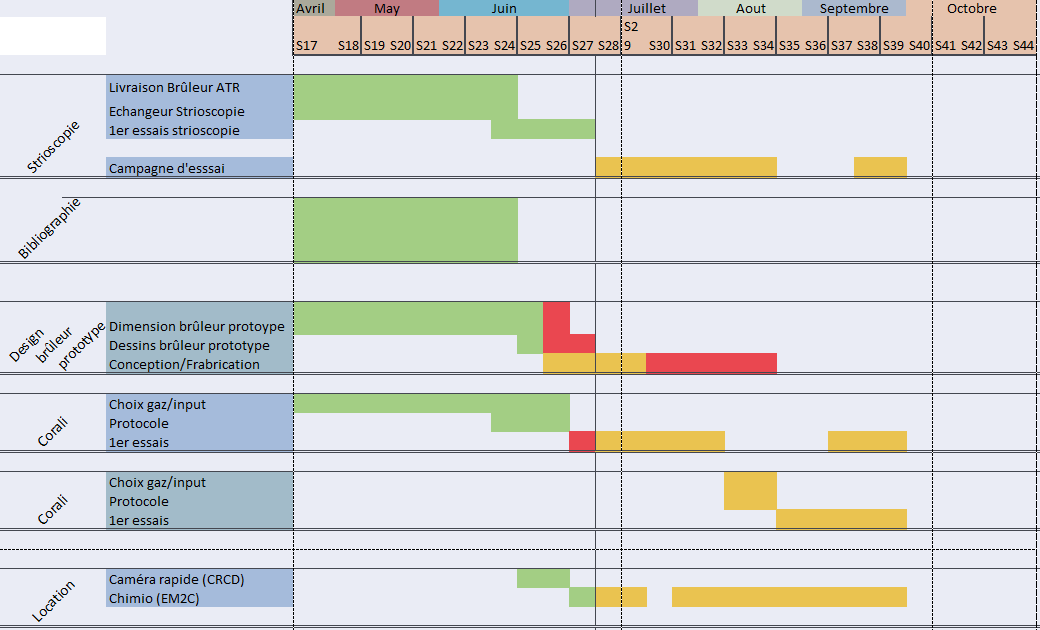
\includegraphics[width=0.9\textwidth]{fig/Gantt_Intermediaire.PNG}
  \caption{Diagramme de Gantt intermédiaire}
 \label{Gantt Int}
\end{figure}
\begin{figure}[!h]
  \centering
\includegraphics[width=0.40\textwidth]
{fig/com/timetable.png}

  \caption{Typical ISO sensitivity}
 \label{fig_Iso_sensitivity_1D}
\end{figure}


Le stage c'est aussi :
\begin{itemize}
\item 60 heures devant le four
\item 2 fois la consommation électrique annuelle d'un couple (sans chauffage)
\item x heures des calcul LES
\item 5 techniciens trop aidants
\item 4 diagnostics optiques différents utilisés
\end{itemize}